\documentclass[11pt,a4paper]{article}

\usepackage[margin=2.5cm]{geometry}
\usepackage[T1]{fontenc}
\usepackage[utf8]{inputenc}
\usepackage{lmodern}
\usepackage{amsmath, amssymb}
\usepackage{booktabs}
\usepackage{graphicx}
\usepackage{listings}
\usepackage{xcolor}
\usepackage[hidelinks]{hyperref}
\usepackage{microtype}
\usepackage[htt]{hyphenat}  % allow long \texttt paths to break

\setlength{\emergencystretch}{3em}

\lstset{
  basicstyle=\ttfamily\footnotesize,
  breaklines=true,
  frame=single,
  framerule=0.3pt,
  rulecolor=\color{gray!50},
  backgroundcolor=\color{gray!6},
  columns=fullflexible,
  keepspaces=true,
  xleftmargin=0.5em,
  aboveskip=0.9em,
  belowskip=0.9em,
}

\usepackage[style=authoryear, backend=biber, maxbibnames=99, sorting=nyt]{biblatex}
\addbibresource{references.bib}

\newcommand{\dial}{\ensuremath{d}}

\title{The Safety Dial on Push-T\\[0.5em]
  \large Constraint-Priority Planning in a Frozen JEPA Latent\\[0.3em]
  \large Diagnosis of the Penalty Sweep, and a Deployment-Time Threshold}
\author{Sachin Mohan \\ Student No. 2699183 \\
  Supervised by Geraud Nangue Tasse \\ University of the Witwatersrand}
\date{20 September 2026}

\begin{document}

\maketitle

\begin{abstract}
This report covers a pilot asked for by the supervisor: make the Safety Dial work against a
hazard placed between the start and the goal, and try a Safe variant of the Cross-Entropy
Method planner. Both are done, on the frozen released \texttt{pusht/lewm} checkpoint with an
unmodified planner.

Three results. First, the earlier penalty sweep, in which every non-zero penalty weight
abandoned the task and drove the pusher out of the arena, is \emph{confounded}. Its dominant
cause was a geometry defect: the hazard box, once inflated by the probe margin, contained the
start state, so every candidate plan was in violation from the first step and the only way to
reduce the penalty was to leave. With the geometry repaired, penalty planning behaves
perfectly reasonably and never leaves the arena at any weight tested. The penalty-fragility
argument should not be rested on that sweep.

Second, Safe CEM, which ranks feasibility before goal progress rather than summing the two,
attains \emph{exactly zero} hazard violations on every episode at every usable dial, nine of
nine. Penalty planning manages zero on only four of nine episodes at non-zero weight, so no
weight achieves it \emph{reliably} and every weight's mean stays positive. This is the
structural difference between a threshold and a weight.

Third, at the most conservative setting the filter broke down in an instructive way: it drove
the pusher off-screen while reporting $80.6\%$ of candidate plans feasible. The arena
constraint had been computed from a learned probe, and a probe trained on in-arena frames
cannot see a pusher that has left the frame. A probe cannot police its own validity domain,
and a conservative threshold pushes the planner directly into that blind spot. Recomputing the
constraint in action space, where it is exact, removes the failure entirely.
\end{abstract}

\tableofcontents

\section{What was asked, and what was done}

The supervisor asked for a small experiment: get the Safety Dial working with a hazard placed
between the start and the goal, and try a Safe CEM. An earlier attempt in
\texttt{experiments/LinearProbeAndAvoidance\_4.ipynb} had not worked.

Everything here runs on the substrate the project already has: the released LeWM checkpoint
\texttt{pusht/lewm} \parencite{maes2026lewm}, frozen, with $192$-dimensional latents, and the
Push-T environment \parencite{chi2023diffusion} as shipped by \texttt{stable\_worldmodel}. The
planner is the stock \texttt{CEMSolver} at its usual settings ($300$ samples, $30$ iterations,
top-$30$ elites, horizon $5$, receding horizon $1$, action block $5$). No world model was
trained. The only new machinery is the cost model that ranks the planner's candidates.

\section{Background: the substrate and the earlier sweep}

\subsection{Push-T as shipped}

Three facts about the environment matter for everything below, and all three were read from
the installed source and then confirmed by direct experiment.

\begin{enumerate}
  \item \textbf{The pusher is kinematic and unbounded.} It is created as a
    kinematic \texttt{pymunk} body and driven by a PD controller
    toward \texttt{agent.position + action * 100}. The clip that would keep it inside the
    arena is present in \texttt{env.step} but \emph{commented out}. Kinematic bodies in pymunk
    ignore collisions, so the pusher passes straight through the arena walls. Driving it with
    $40$ steps of action $(-1,-1)$ put it at $(-1380.9, -1313.1)$, and $40$ steps of $(+1,+1)$
    returned it to $(224.7, 292.6)$.
  \item \textbf{The block is walled in.} The T-block is a dynamic body enclosed by static
    segments spanning $(5,5)$ to $(506,506)$. Pushed into the left wall it stops with its
    centre near $x = 48$ and cannot leave.
  \item \textbf{The dynamics are quasi-static.} The space has zero gravity and
    \texttt{damping = 0}, which in pymunk removes velocity essentially immediately. Verified:
    a body given velocity $100$ is at rest after one step. The block moves only while it is
    being pushed.
\end{enumerate}

A consequence worth recording for the wider project: Push-T has \emph{no absorbing states}.
The block cannot be lost, the pusher is fully actuated and can pass through walls, and the
dynamics are quasi-static, so every configuration remains mutually reachable. Push-T can
support a hazard-avoidance study like this one, but it cannot support a study of binary
irreversibility. There, irreversibility would have to be reframed as a graded cost-to-return.

\subsection{The earlier penalty sweep}

The previous attempt swept a weight $\lambda$ in a scalarised cost
$C = \text{goal} + \lambda \cdot \text{hazard}$ over seven values and five seeds. Every
non-zero $\lambda$ produced a final block error of $70.7$ pixels, which was exactly the
start-to-goal block distance, meaning the block had never moved, and every non-zero $\lambda$
drove the pusher out of the arena. That outcome was recorded in the project notes as a clean
demonstration of penalty fragility.

\section{Diagnosis: three causes, one dominant}

\subsection{Cause 1: the start was inside the inflated hazard}

The helper \texttt{hazardSweep.calibrate\_box} places the hazard on the baseline path and
sorts candidates by descending baseline violation, but it never checks that the start state
clears the box once the probe margin is added. The box it selected was
$(2, 82, 83, 163)$. Inflated by the planning margin of $35.5$ pixels this becomes
$(-33.5, 117.5, 47.5, 198.5)$, which \emph{contains} the pusher start $(70, 70)$.

Every candidate plan was therefore in violation from step zero. The penalty term was a large
near-constant offset that the planner could not reduce by planning better, only by leaving the
region entirely, and because the pusher is unbounded it could do exactly that at no cost. The
notebook contains a manual workaround, a hardcoded box annotated as clearing the start by
$12.5$ pixels after margin, which shows the problem had been half-noticed.

\subsection{Cause 2: the planner could escape}

Given an infeasible objective, fleeing the arena drives any hazard penalty to zero for free.
This is a direct consequence of the kinematic, unclipped pusher described above. It is better
understood as an \emph{amplifier} of cause 1 than as an independent cause, for reasons the
results make clear.

\subsection{Cause 3: a weight is not a threshold}

With a scalarised cost there is no notion of a feasible plan. The weight $\lambda$ carries no
units, its useful range depends on the relative scales of the goal and hazard terms, and it
must be re-swept whenever either changes. An operator cannot be handed $\lambda$ and told what
it means. This is the conceptual reason the dial has to be a threshold.

\section{Method}

\subsection{Safe CEM by constraint-priority ranking}

The stock \texttt{CEMSolver} selects its elite set with
\texttt{torch.topk(costs, largest=False)}, which is a pure scalar ranking. Constraint-priority
ranking can therefore be encoded in the scalar itself, and the upstream solver needs no
modification at all:
\[
  C_j =
  \begin{cases}
    g_j & \text{if } v_j \le 0 \quad \text{(feasible)},\\[2pt]
    \big(\max_{k:\, v_k \le 0} g_k\big) + 1 + v_j & \text{otherwise},
  \end{cases}
\]
where $g_j$ is the world model's goal cost for candidate $j$ and $v_j \ge 0$ is its predicted
constraint violation in pixels. Every feasible candidate then sorts ahead of every infeasible
one; feasible candidates sort among themselves by goal progress; and infeasible candidates
sort by violation magnitude. This is the constraint-priority ranking of MPC-RCE
\parencite{liu2020constrained}, which is already in the project's reading list.

Two details are load-bearing. The infeasible branch must stay \emph{graded} rather than
constant, because CEM sets its next variance from \texttt{topk\_candidates.std(dim=1)}: a
constant cost makes the elite set arbitrary and the search collapses. And when no candidate is
feasible the offset falls back to the global maximum, so the ranking degrades gracefully to
pure constraint minimisation, which is the behaviour wanted when the planner must first
recover feasibility.

\subsection{The dial}

The dial $\dial$ is the required clearance, in pixels, by which the hazard box is inflated for
the feasibility test. It is set at deployment on one frozen model. Violations are always
\emph{measured} against the true, uninflated box using simulator state, never against the
inflated box the planner reasons about.

\subsection{Hazard placement}

A hazard placement has to satisfy two conditions at once, and each existing helper supplies
only one. Placing the box on the observed baseline route guarantees there is something to
avoid but does not guarantee clearance, which is cause 1. Placing it on the straight line
between start and goal guarantees clearance but not relevance: measured directly, such a box
had a baseline violation fraction of $0.00$, so the sweep would have measured nothing.

\texttt{safeCEM.calibrate\_box\_on\_path} requires both, searching placements along the route
the unconstrained planner actually took and rejecting any that fail clearance at the widest
dial. Its candidate table reproduces the original defect mechanically: the highest-violation
placements are exactly the ones that fail clearance.

\begin{center}
\footnotesize
\begin{tabular}{rrrrl}
\toprule
frac & half & baseline viol. & clear & box \\
\midrule
0.70 & 40 & 0.46 & \textbf{False} & $(214, 294, 313, 393)$ \\
0.50 & 40 & 0.40 & \textbf{False} & $(195, 275, 307, 387)$ \\
0.30 & 50 & 0.14 & True  & $(30, 130, 149, 249)$ \quad chosen \\
0.30 & 30 & 0.10 & True  & $(50, 110, 169, 229)$ \\
\bottomrule
\end{tabular}
\end{center}

\section{Experimental setup}

The pusher starts at $(40, 40)$ with a goal pose at $(250, 310)$; the block starts at
$(300, 310)$ and must reach $(360, 310)$, a displacement of $60$ pixels. The block and its
goal sit well clear of the hazard, deliberately: if the block were inside the hazard the
pusher could not touch it without violating, safety and task would be irreconcilable, and
every setting would degenerate to abandoning the task. Here a tighter dial costs a detour
rather than the task.

The calibrated hazard is $(30, 130, 149, 249)$, which the unconstrained planner enters on
$14\%$ of steps. Start and goal clear the box at every dial tested, by $108.7$ and $119.9$
pixels at $\dial = 0$ and still by $48.7$ and $59.9$ pixels at $\dial = 60$. A safe route
exists comfortably: the best detour is $367.7$ pixels against a budget of $1062$ pixels.

Three arms share an identical constraint definition so that any difference is attributable to
the ranking rule alone:

\begin{itemize}
  \item \textbf{penalty-noarena}: $C = g + \lambda v_{\text{hazard}}$, with the escape route
    left open.
  \item \textbf{penalty}: $C = g + \lambda (v_{\text{hazard}} + v_{\text{arena}})$.
  \item \textbf{safe}: constraint-priority ranking with dial $\dial$.
\end{itemize}

Three seeds per setting, $50$ environment steps per episode. Reported metrics are the fraction
of steps with the pusher inside the true hazard box, the final block error in pixels, the
fraction of steps outside the arena, and the fraction of candidate plans the planner believed
feasible at the last CEM iteration of each replan.

\paragraph{Provenance, which matters for one row of the results.} This sweep was run
\emph{before} the action-space arena constraint of Section~\ref{sec:fix} existed, so its arena
constraint was the probe-based one throughout. That variant is now no longer the default, so a
plain rerun will \emph{not} reproduce the $\dial = 60$ breakdown, which is a property of the
probe-based constraint specifically. The exact table is reproduced with
\texttt{safe\_dial\_pusht.py -{}-quick -{}-seeds 3 -{}-probe-arena}, and the committed
\texttt{results.json} records which variant produced it in its
\texttt{arena\_constraint\_mode} field. This does not affect the penalty arms, where the arena
term never binds because the out-of-bounds fraction is zero at every weight.

\section{Results}

\begin{table}[h]
\centering
\begin{tabular}{lrrrr}
\toprule
\multicolumn{5}{l}{\textbf{Penalty CEM}, arena constrained} \\
\midrule
$\lambda$ & viol. fraction & block err. (px) & out of bounds & feasible \\
\midrule
0    & $0.188 \pm 0.097$ & $11.2 \pm 0.6$ & 0.000 & 0.590 \\
0.1  & $0.073 \pm 0.031$ & $7.8 \pm 2.1$  & 0.000 & 0.857 \\
1    & $0.020 \pm 0.028$ & $\mathbf{4.9 \pm 1.7}$ & 0.000 & 0.958 \\
10   & $0.011 \pm 0.015$ & $7.9 \pm 2.4$  & 0.000 & 0.976 \\
\midrule
\multicolumn{5}{l}{\textbf{Safe CEM}, dial $\dial$ in pixels of clearance} \\
\midrule
$\dial$ & viol. fraction & block err. (px) & out of bounds & feasible \\
\midrule
0   & $\mathbf{0.000 \pm 0.000}$ & $9.0 \pm 1.1$  & 0.000 & 0.974 \\
20  & $\mathbf{0.000 \pm 0.000}$ & $11.9 \pm 1.9$ & 0.000 & 0.964 \\
40  & $\mathbf{0.000 \pm 0.000}$ & $6.7 \pm 2.0$  & 0.000 & 0.796 \\
60  & $0.000 \pm 0.000$ & $60.0 \pm 0.0$ & \textbf{0.953} & 0.806 \\
\bottomrule
\end{tabular}
\caption{Three seeds per setting. Violations are measured against the true hazard box from
simulator state. The $\dial = 60$ row is a breakdown, discussed in
Section~\ref{sec:breakdown}: its zero violation is achieved vacuously, by leaving the arena.}
\label{tab:main}
\end{table}

\begin{figure}[htbp]
\centering
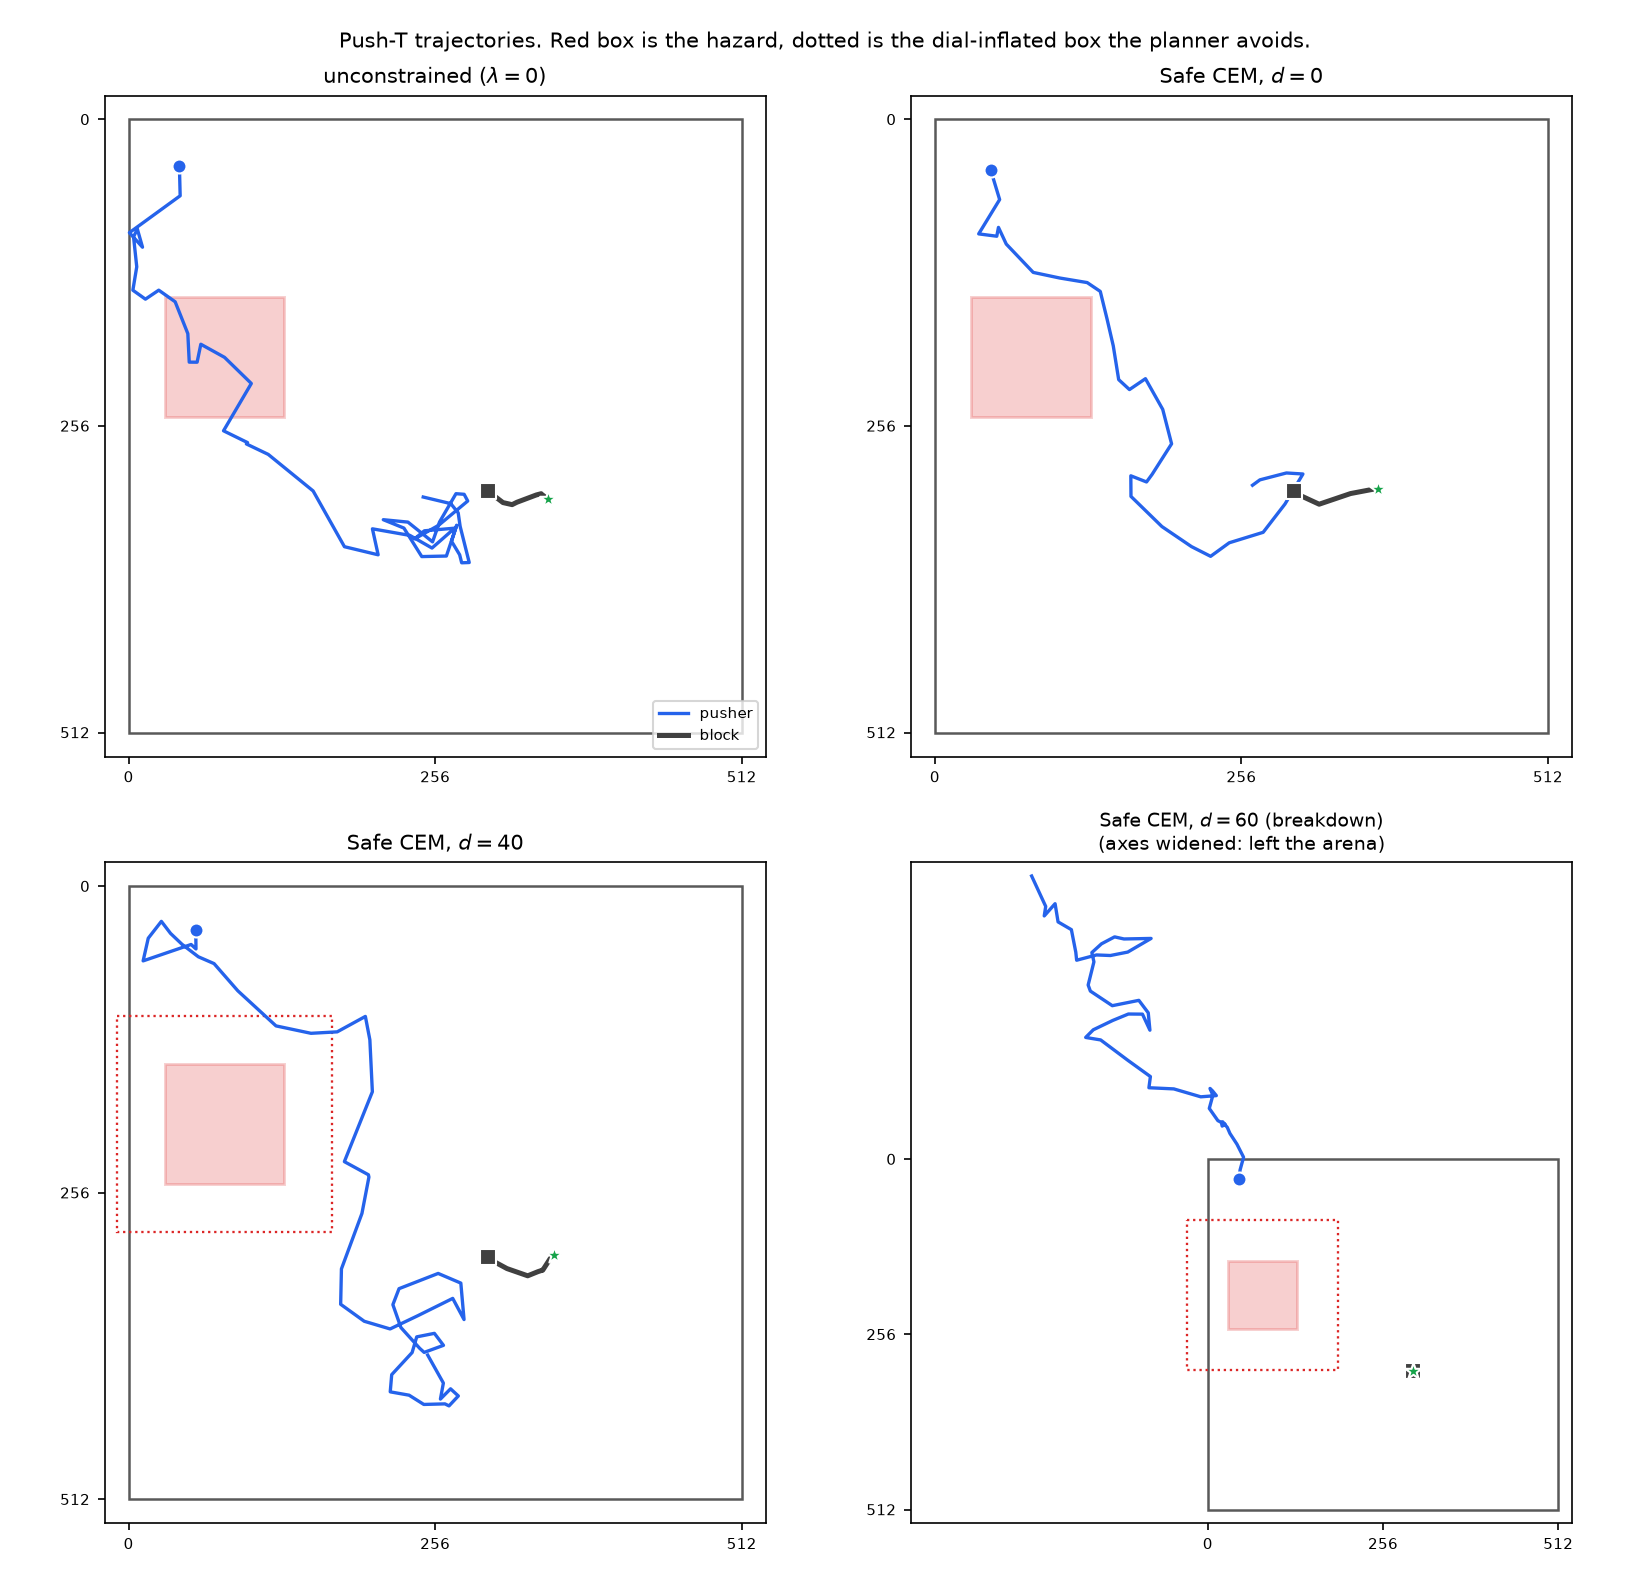
\includegraphics[width=0.92\textwidth]{figures/trajectories.png}
\caption{What the planner actually did, one seed per panel. The shaded red square is the true
hazard; the dotted square is the dial-inflated region the planner reasons about. The
unconstrained planner drives straight through the hazard. At $\dial = 0$ the pusher curves
around it, and at $\dial = 40$ it gives the inflated region a wide berth, in both cases still
reaching the block and pushing it to the goal (star). At $\dial = 60$ the axes have to be
widened because the pusher leaves the arena entirely and the block is never touched.}
\label{fig:traj}
\end{figure}

\begin{figure}[htbp]
\centering
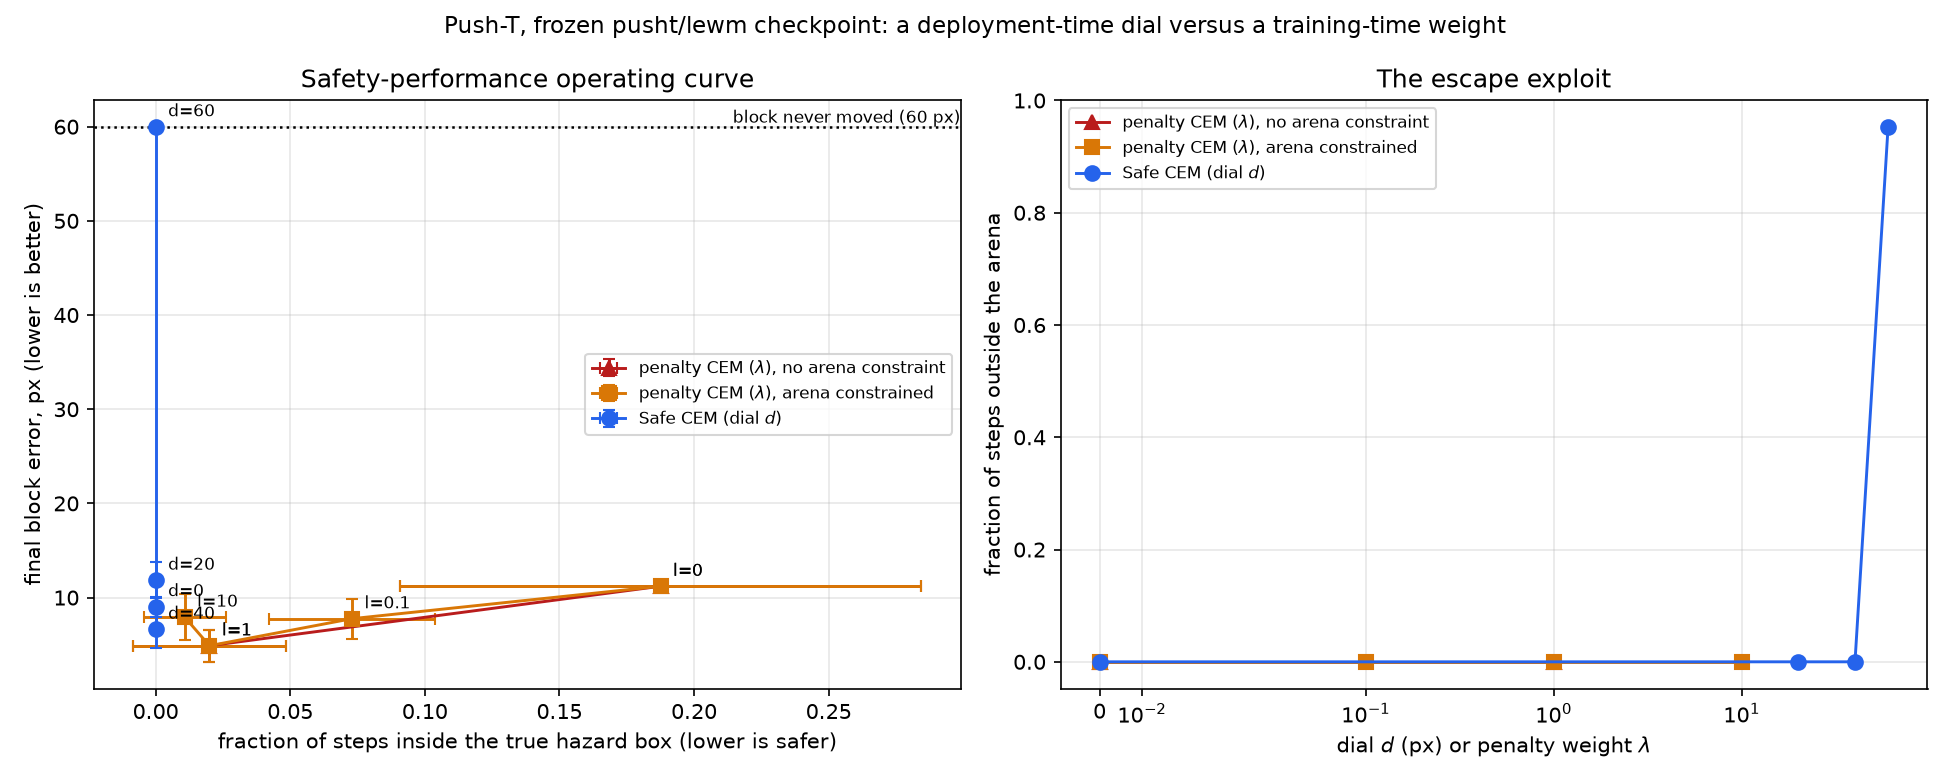
\includegraphics[width=\textwidth]{figures/tradeoff.png}
\caption{Left: the safety-performance operating curve. Safe CEM sits on the zero-violation
axis while the penalty curve approaches it without reaching it. Right: the escape exploit,
which is flat at zero everywhere except the $\dial = 60$ breakdown.}
\label{fig:tradeoff}
\end{figure}

\begin{figure}[htbp]
\centering
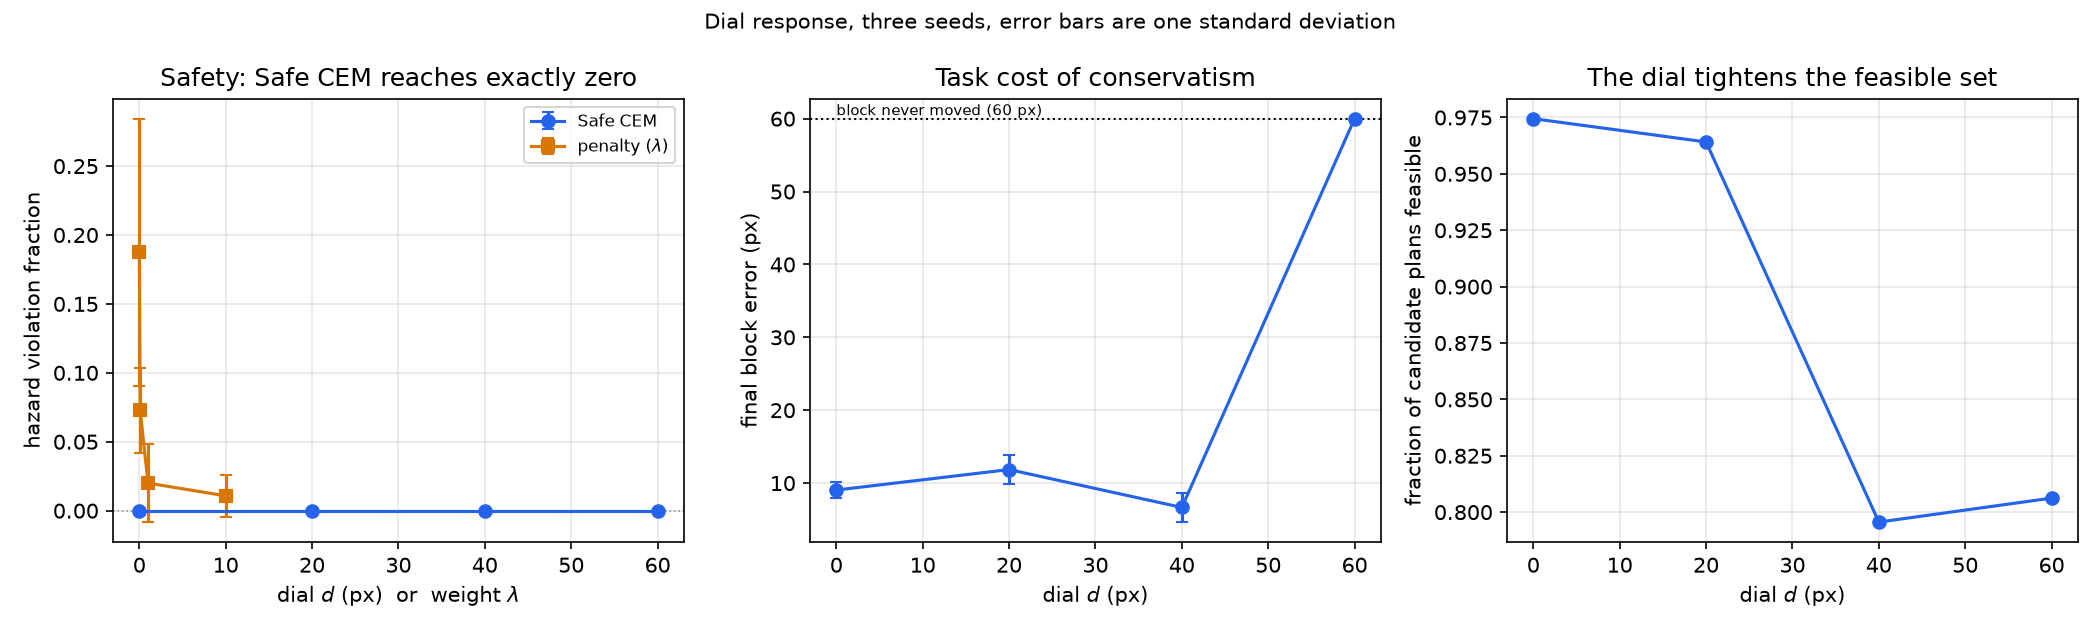
\includegraphics[width=\textwidth]{figures/dial_response.png}
\caption{Dial response. Left: Safe CEM is flat on zero at every usable setting while the
penalty curve is asymptotic to it, never touching. Note the two series share an axis but not
units, pixels of clearance against a dimensionless weight, which is itself the point. Centre:
the task cost, flat within seed noise until the $\dial = 60$ breakdown. Right: the dial does
bite internally, tightening the fraction of candidate plans the planner deems feasible from
$0.974$ to $0.796$ across $\dial = 0$ to $40$.}
\label{fig:dial}
\end{figure}

\subsection{Safe CEM reaches zero; no weight does}

Safe CEM attains exactly zero violations on \emph{every} episode at
$\dial \in \{0, 20, 40\}$, nine of nine. Penalty planning reaches zero on only four of nine
episodes at non-zero weight, so its seed means never vanish: $\lambda = 10$ averages $0.011$
because one of its three seeds violates on $3.2\%$ of steps.

\begin{center}
\footnotesize
\begin{tabular}{lccc c}
\toprule
setting & \multicolumn{3}{c}{per-episode violation fraction} & episodes at zero \\
\midrule
$\lambda = 0$    & 0.140 & 0.323 & 0.100 & 0 of 3 \\
$\lambda = 0.1$  & 0.114 & 0.040 & 0.065 & 0 of 3 \\
$\lambda = 1$    & 0.000 & 0.060 & 0.000 & 2 of 3 \\
$\lambda = 10$   & 0.000 & 0.000 & 0.032 & 2 of 3 \\
\midrule
$\dial = 0$      & 0.000 & 0.000 & 0.000 & \textbf{3 of 3} \\
$\dial = 20$     & 0.000 & 0.000 & 0.000 & \textbf{3 of 3} \\
$\dial = 40$     & 0.000 & 0.000 & 0.000 & \textbf{3 of 3} \\
\bottomrule
\end{tabular}
\end{center}

The difference is structural rather than a matter of tuning. A weighted sum will accept a
small violation in exchange for a large enough goal improvement, so whether any particular
episode comes out clean depends on the trajectory it happens to find; constraint-priority
ranking never makes that exchange, so it is clean every time. The claim that survives the data
is therefore about \emph{reliability}, not about zero being unreachable by a penalty: it is
reachable, just not dependably. The price is about $4$ pixels of task accuracy against the
best-tuned weight ($9.0$ against $4.9$ pixels).

Note also that the penalty arm's task metric is \emph{non-monotone} in $\lambda$: it improves
to $4.9$ pixels at $\lambda = 1$ and degrades again to $7.9$ at $\lambda = 10$. The good
operating point is interior and can only be found by sweeping. The dial has no such interior
optimum to find.

\subsection{The penalty-fragility result is confounded}

With the geometry repaired, penalty planning is not fragile here at all. Violation falls
monotonically in $\lambda$ (Spearman $-1.0$), and the pusher stays inside the arena at
\emph{every} weight tested, with an out-of-bounds fraction of exactly $0.000$. That holds even
in the \texttt{penalty-noarena} arm, which has no arena constraint whatsoever and so leaves
the escape route completely open. Indeed the two penalty arms agree exactly at $\lambda = 0$
and $\lambda = 1$, because the arena term is never active and therefore never binds.

The earlier catastrophic sweep is therefore explained by cause 1, not by any inherent
fragility of penalty methods. A referee who reproduces that sweep from a feasible start will
find that $\lambda = 1$ works. The project's motivation section should rest on the dial's
interpretability and its zero-violation guarantee instead.

\subsection{The breakdown at the widest dial, and why a probe cannot enforce an arena constraint}
\label{sec:breakdown}

At $\dial = 60$ every seed collapses in the same way. The block never moves: the final block
error is $60.0 \pm 0.0$ pixels, exactly the start-to-goal block distance. The pusher is
outside the arena for $47$ to $48$ of $50$ steps, reaching $x = -276$ and $y = -562$. The
reported violation of $0.000$ is achieved \emph{vacuously}, by leaving the arena so the true
box is never entered. This is the original pathology returning, at the setting where the
constraint finally becomes tight enough that escape is the cheapest way to satisfy it.

The arena constraint did not prevent this, and structurally could not have. It was evaluated
on $\text{probe}(\hat z)$, and the probe is a regressor trained on in-arena frames. Once the
pusher truly leaves the $512$ pixel arena it is not visible in the $224$ pixel frame at all,
so no encoder output carries its position and the probe's estimate is uninformative. The
planner sincerely reported $80.6\%$ of candidates feasible while driving off-screen.

The general statement is worth keeping, because it is not specific to this pilot:
\emph{a learned probe cannot police its own validity domain, and a conservative threshold
pushes the planner directly toward the blind spot}, since leaving the domain is the cheapest
way to satisfy a tight constraint. This is a concrete, measured instance of the failure that
uncertainty-aware latent safety filters such as UNISafe \parencite{seo2025unisafe} exist to
address.

\subsection{The fix, and its validation}
\label{sec:fix}

The correct constraint is computed in \emph{action space}, where it is exact. The Push-T
pusher is position-controlled: \texttt{env.step} sets the PD target to
\texttt{agent.position + action * 100} and runs ten substeps, which is enough to reach it. So
the commanded trajectory is a closed-form function of the candidate action sequence and the
current position, involving no world model and no probe. This is
\texttt{safeCEM.commanded\_positions}, enabled by \texttt{action\_space\_arena=True}.

A paired re-run at $\dial = 60$, executing both constraint variants on the same three seeds
with nothing else changed (\texttt{experiments/scripts/validate\_arena\_fix.py -{}-both}), also
independently reproduced the breakdown before fixing it:

\begin{center}
\begin{tabular}{llrrrrr}
\toprule
constraint & seed & viol. & block err. (px) & out of bounds & block moved (px) & feasible \\
\midrule
probe-based   & 0 & 0.000 & 60.0 & 0.960 & 0.0  & 0.805 \\
probe-based   & 1 & 0.000 & 60.0 & 0.960 & 0.0  & 0.805 \\
probe-based   & 2 & 0.000 & 60.0 & 0.940 & 0.0  & 0.808 \\
\midrule
action-space  & 0 & 0.000 & 9.4  & 0.000 & 66.8 & 0.613 \\
action-space  & 1 & 0.000 & 15.8 & 0.000 & 67.8 & 0.692 \\
action-space  & 2 & 0.000 & 24.8 & 0.000 & 84.0 & 0.644 \\
\bottomrule
\end{tabular}
\end{center}

\begin{figure}[htbp]
\centering
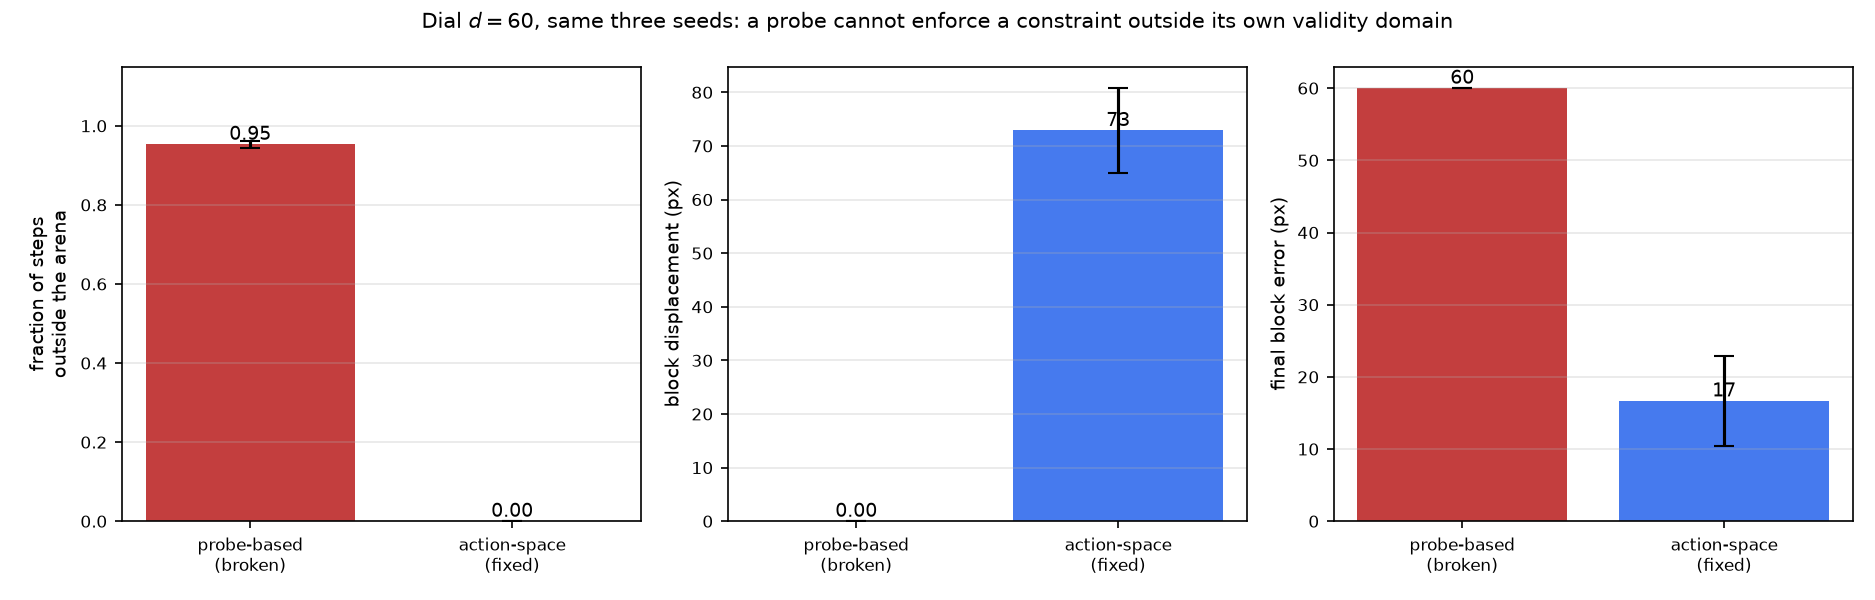
\includegraphics[width=\textwidth]{figures/arena_fix.png}
\caption{Paired comparison at $\dial = 60$, three seeds each. With the probe-based constraint
the pusher is outside the arena for $95\%$ of steps and the block never moves, so the final
error equals the full start-to-goal distance. With the action-space constraint the pusher
stays inside, the block is pushed $67$ to $84$ pixels, and the final error falls accordingly.}
\label{fig:arenafix}
\end{figure}

\begin{figure}[htbp]
\centering
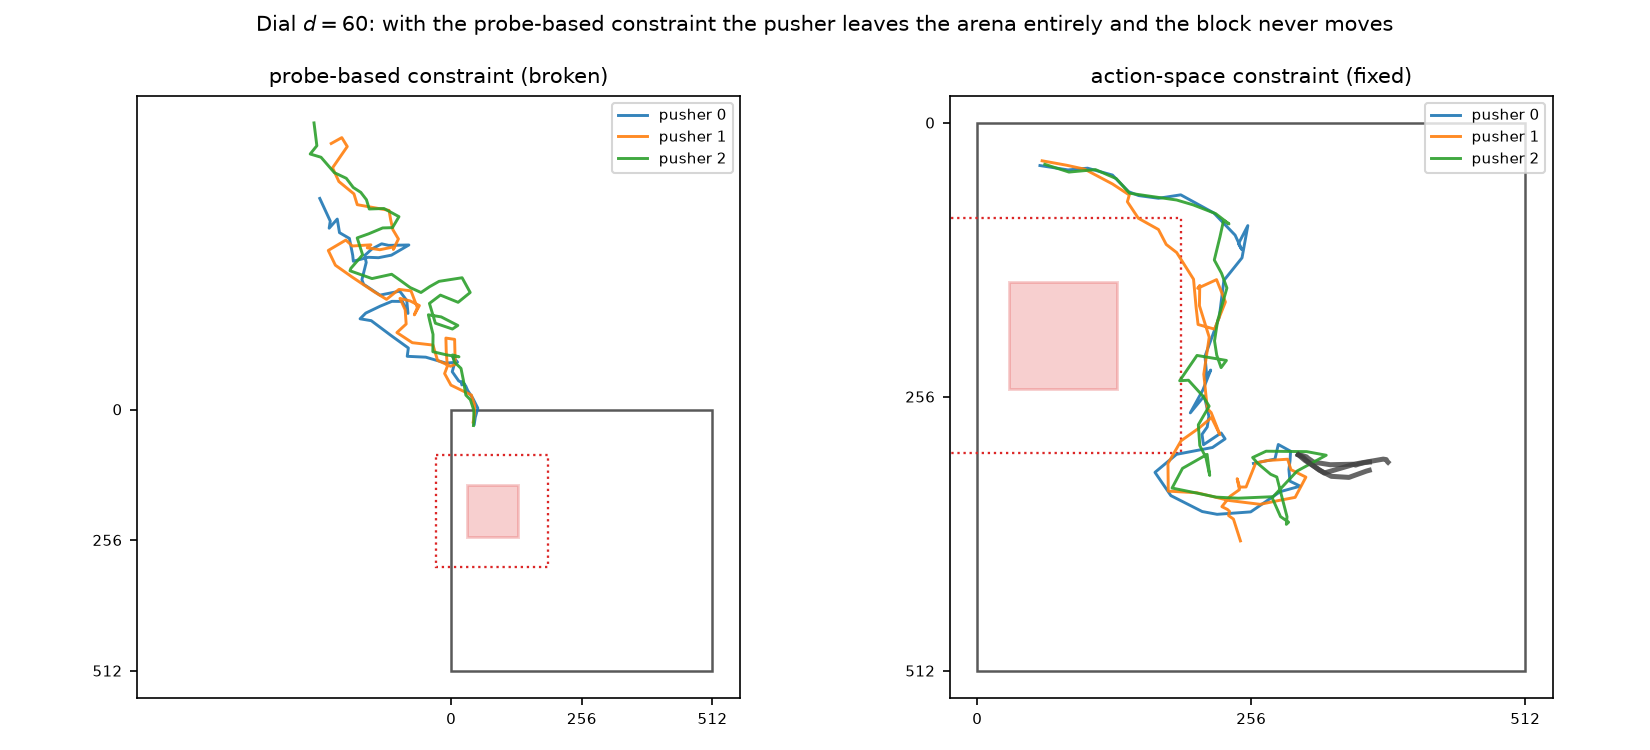
\includegraphics[width=\textwidth]{figures/arena_fix_traj.png}
\caption{The same comparison as trajectories. Left, the planner escapes to roughly
$x = -270$, $y = -560$, far outside the arena drawn in grey, while reporting most of its
candidate plans feasible. Right, with the constraint computed in action space it stays inside
and completes the push.}
\label{fig:arenafixtraj}
\end{figure}

Out-of-bounds falls from $0.953$ to $0.000$, the block moves $67$ to $84$ pixels instead of
not at all, and the block error falls from $60.0$ to between $9.4$ and $24.8$ pixels.
Violation remains zero, but now genuinely rather than vacuously. The fraction of candidates
believed feasible drops from $0.806$ to about $0.65$, which is the honest figure: the
constraint is real now, so fewer plans satisfy it. The earlier $0.806$ was inflated by the
probe's blindness.

The pragmatic alternative, for anyone who prefers not to change the planner, is to restore the
commented-out action clip in \texttt{env.step}, which makes the arena physically inescapable.

\section{What this does and does not establish}

\paragraph{Established.} Safe CEM works on this substrate, attains zero violations where no
penalty weight does, and its dial is expressed in interpretable units on a single frozen
model. The earlier penalty-fragility result is confounded and should not be used as
motivation. A probe-derived constraint cannot bound the probe's own validity domain, and the
action-space constraint fixes the resulting failure.

\paragraph{Not established.} Hypothesis H4, a monotone safety-performance trade-off, is
\emph{not} demonstrated by this run. The safety axis saturates at zero for every usable dial,
and block error is non-monotone within seed noise ($9.0$, $11.9$, $6.7$ pixels at $\pm 1$ to
$2$). The reason is visible in the setup: the detour has $694$ pixels of slack against a
$1062$ pixel budget, so tightening the dial costs almost nothing. The dial does bite on the
planner's internal feasible set, which falls monotonically from $0.974$ to $0.964$ to $0.796$,
but that is an internal diagnostic and not a trade-off curve.

The validation run hints the trade-off is real once the arena constraint is exact, with mean
block error of $9.0$ pixels at $\dial = 0$ against $16.7$ pixels at $\dial = 60$, both at zero
violation. Seed variance is large, so this should not be quoted before a fuller run.

\paragraph{Scope.} This is a hazard-avoidance pilot with an extrinsic, hand-placed hazard
region, not a study of irreversibility. Push-T has no absorbing states, so it cannot host the
latter. The probe supervises a generic physical quantity, the pusher position, and never the
safety concept itself.

\section{Next steps}

\begin{enumerate}
  \item \textbf{Gate geometry.} Replace the single box with two boxes separated by a gap of
    width $w$. For $\dial < w/2$ the planner passes through; for $\dial > w/2$ the gate closes
    and it must detour or give up. This produces a sharp, interpretable dial response and a
    genuine trade-off, and it is still a hazard between start and goal.
  \item \textbf{Full grid rerun} with \texttt{action\_space\_arena=True}, the complete dial
    range and five seeds, to settle whether the task-axis trade-off is real.
  \item \textbf{Block-space hazard.} The probe currently decodes pusher position only.
    Constraining the \emph{block} instead would be closer to a real safety specification and
    needs a block position and orientation probe, with orientation regressed as
    $(\sin\theta, \cos\theta)$ because it is periodic.
  \item \textbf{Revise the preliminary-evidence section} of the proposal in light of
    Section~4.2.
\end{enumerate}

\section{Reproduction}

\begin{lstlisting}[language=bash]
# Smoke test: one episode per arm
uv run python experiments/scripts/safe_dial_pusht.py --smoke

# The run reported here: reduced grid, three seeds
uv run python experiments/scripts/safe_dial_pusht.py --quick --seeds 3

# Figure
uv run python experiments/scripts/plot_safe_dial.py
\end{lstlisting}

The probe is trained and cached to \texttt{data/probes/pusher\_mlp.pt} on first use, which
takes about two minutes; later runs load it.

Because \texttt{outputs/} and \texttt{data/} are gitignored and this machine is not a
persistent volume, every artifact behind this report is committed under
\texttt{docs/safeDial/} instead: \texttt{results/results.json} and
\texttt{results\_states.npz} for the sweep, \texttt{results/arena\_fix.json} and
\texttt{arena\_fix\_states.npz} for the paired dial-60 run, and
\texttt{latex/figures/} for every figure. Each JSON carries a provenance note recording the
command that produced it.

\appendix

\section{Environment notes that cost real time}

\paragraph{The container CPU quota is not \texttt{nproc}.} This machine reports
\texttt{/sys/fs/cgroup/cpu.max} of \texttt{1152000 100000}, that is $11.52$ CPUs, while
\texttt{nproc} and \texttt{os.sched\_getaffinity} both report $96$. Torch sizes its intra-op
thread pool from the affinity mask, so it spawns $96$ threads into $11.5$ cores and thrashes.
The symptom is a CEM solve taking $15$ seconds instead of $1$, with the GPU at $0$ to $4$
percent throughout and \texttt{nr\_throttled} climbing in \texttt{cpu.stat}. Cap the pools
before importing torch. Measured at $10$ CEM iterations, two solves: bare goal cost $4.4$
seconds, the new cost model $6.6$ seconds, the older notebook cost model $15.8$ seconds, so
the constraint machinery is cheap and the thread thrash was the real cost.

\paragraph{Never fancy-index the pixels array.} Contiguous HDF5 reads run at about $19{,}000$
frames per second; a sorted scattered fancy-index runs at about $46$, a factor of $415$. Read
contiguous spans at spread offsets.

\paragraph{Encode rate.} End to end, including cold reads and host-to-device transfer, the
encoder sustains about $939$ frames per second, so a full $2.34$M frame latent bank takes
roughly $44$ minutes. A GPU-only microbenchmark suggesting $8{,}000$ frames per second is not
the rate obtained in practice.

\paragraph{Latent-start rollouts need no new code.} The installed
\texttt{LeWM.rollout} in \texttt{stable\_worldmodel} caches the initial embedding
(\texttt{if 'emb' not in info}), which the older copy in \texttt{third\_party/le-wm/jepa.py}
does not. Supplying \texttt{info['emb']} of shape $(B, S, H, D)$ together with any tensor whose
dimension $2$ equals $H$ starts a rollout from a latent directly. Measured on the GPU here,
$1024$ action samples over $10$ latent steps cost $52$ milliseconds and $0.24$ GB. The action
encoder takes $10$ inputs, which is the action block of $5$ times the action dimension of $2$,
and this is why \texttt{action\_block} must stay at $5$.

\paragraph{Push-T state columns.} From the simulator's \texttt{\_get\_obs}, the seven-dimensional
state is pusher $x$, pusher $y$, block $x$, block $y$, block $\theta$ taken modulo $2\pi$, and
pusher velocity $x$ and $y$. The last two are the pusher's velocity, not unknown extras.

\printbibliography

\end{document}
